\colorlet{species background color}{black!15}
\tikzset{
    x={1pt},
    y={-1pt},
    species background/.style={
        fill=species background color,
        draw=species background color,
        line width={1pt},
    },
    species label/.style={
        font=\bfseries,
        midway,
        anchor=west,
        align=left,
        xshift=10,
    },
    branch/.style={
        draw={#1},
        line width={0.5pt},
    },
    transfer branch/.style={
        branch={#1},
        -Stealth,
    },
    loss/.style={
        draw={#1}, cross out, thick,
        line width={0.5pt},
        inner sep=0pt,
        outer sep=0pt,
        minimum width={3},
        minimum height={3},
    },
    extant gene/.style 2 args={
        circle, fill={#1},
        outer sep=0pt, inner sep=0pt,
        minimum size={3},
        label={
            [font={\color{#1}},
                align=justify,
                inner xsep=4pt, inner ysep=0pt,
                outer xsep=0pt, outer ysep=0pt]
            right:#2
        },
    },
    extant gene/.default={black}{},
    branch node/.style={
        draw={#1}, fill={species background color!50!white},
        align=center,
        font={\color{#1}},
        outer sep=0pt, inner xsep=0pt, inner ysep=2pt,
        line width={0.5pt},
    },
    branch node/.default={black},
    speciation/.style={
        branch node={#1}, rectangle, rounded corners,
        inner xsep=4pt,
        minimum width={8},
        minimum height={8},
    },
    duplication/.style={
        branch node={#1}, rectangle,
        inner xsep=4pt,
        minimum width={8},
        minimum height={8},
    },
    horizontal gene transfer/.style={
        branch node={#1}, chamfered rectangle,
        chamfered rectangle sep={8 / 2.4},
        inner xsep=2pt,
        inner ysep=-1pt,
        minimum width={8},
        minimum height={8},
    },
}
\definecolor{reccolor0}{HTML}{000000}
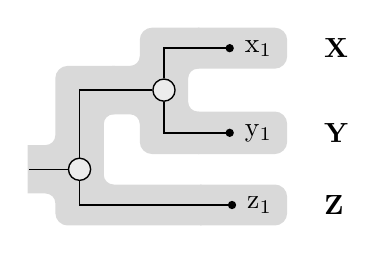
\begin{tikzpicture}
% background
\path[species background] (30.5,13.80997) [rounded corners={4pt}] -- (10,13.80997) -- (10,42.41996) [sharp corners] -- (0,42.41996) -- (0,58.91996) [rounded corners={4pt}] -- (10,58.91996) -- (10,70.47993) [sharp corners] -- (61.84,70.47993) -- (61.84,56.66996) [rounded corners={4pt}] -- (26.5,56.66996) -- (26.5,30.30997) [sharp corners] -- (30.5,30.30997) -- cycle;
\path[species background] (61.0,0) [rounded corners={4pt}] -- (40.5,0) -- (40.5,13.80997) [sharp corners] -- (30.5,13.80997) -- (30.5,30.30997) [rounded corners={4pt}] -- (40.5,30.30997) -- (40.5,44.66996) [sharp corners] -- (61.0,44.66996) -- (61.0,30.30997) [rounded corners={4pt}] -- (57.0,30.30997) -- (57.0,13.80997) [sharp corners] -- (61.0,13.80997) -- cycle;
\path[
                species background,
                rounded corners={4pt},
            ] (61.0,0) -- (92.763,0) -- node[species label] {X} (92.763,13.80997) -- (61.0,13.80997);
\path[
                species background,
                rounded corners={4pt},
            ] (61.0,30.30997) -- (92.763,30.30997) -- node[species label] {Y} (92.763,44.66996) -- (61.0,44.66996);
\path[
                species background,
                rounded corners={4pt},
            ] (61.84,56.66996) -- (92.763,56.66996) -- node[species label] {Z} (92.763,70.47993) -- (61.84,70.47993);
% species
% gene branches
\path[branch={reccolor0}] (14,50.66996) -- (0,50.66996);
\draw[branch={reccolor0}] (30.5,22.05997) -| (18.25,46.41996) (18.25,54.91996) |- (61.84,63.574945);
\path[branch={reccolor0}] (44.5,22.05997) -- (30.5,22.05997);
\draw[branch={reccolor0}] (61.0,6.904985) -| (48.75,17.80997) (48.75,26.30997) |- (61.0,37.489965000000005);
\path[branch={reccolor0}] (71.0,6.904985) -- (61.0,6.904985);
\path[branch={reccolor0}] (71.0,37.489965000000005) -- (61.0,37.489965000000005);
\path[branch={reccolor0}] (71.84,63.574945) -- (61.84,63.574945);
% gene transfers
% events
\node[speciation={reccolor0}] at (18.25,50.66996) {};
\node[speciation={reccolor0}] at (48.75,22.05997) {};
\node[extant gene={reccolor0}{x\textsubscript{1}}] at (72.5,6.904985) {};
\node[extant gene={reccolor0}{y\textsubscript{1}}] at (72.5,37.489965000000005) {};
\node[extant gene={reccolor0}{z\textsubscript{1}}] at (73.34,63.574945) {};
\end{tikzpicture}
